% BAC 2025 D - Exercice 3
% Courbe de f(x) = (e^x - x - 2)e^{-x} = 1 - (x+2)/e^x
% Avec asymptote horizontale y = 1 et tangente en -∞

\documentclass[border=5pt]{standalone}
\usepackage{pgfplots}
\usepackage{amsmath}
\usepackage{amssymb}

\begin{document}

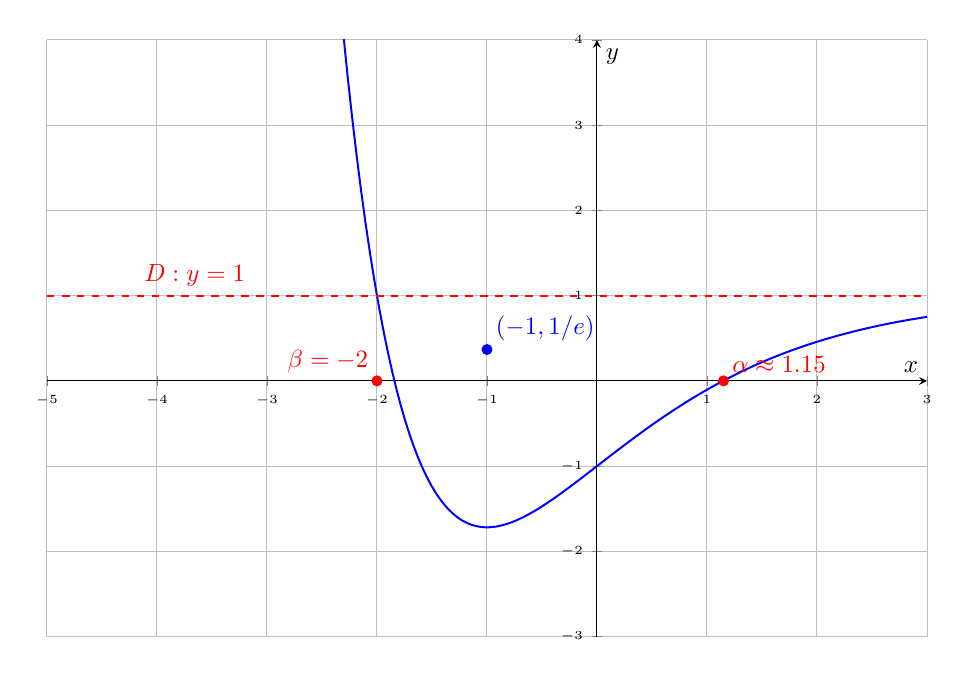
\begin{tikzpicture}[scale=0.9]
\begin{axis}[
    width=14cm,
    height=10cm,
    axis lines=center,
    xlabel=$x$,
    ylabel=$y$,
    xmin=-5, xmax=3,
    ymin=-3, ymax=4,
    grid=major,
    samples=200,
    legend pos=outer north east,
    tick label style={font=\tiny}
]

% Function f(x) = (e^x - x - 2)e^{-x}
\addplot[blue, thick, domain=-5:3] {(exp(x) - x - 2)*exp(-x)} 
    node[pos=0.7, above left] {$\Gamma$};

% Asymptote horizontale y = 1
\addplot[red, dashed, thick, domain=-5:3] {1} 
    node[pos=0.1, above right] {$D: y=1$};

% Asymptote oblique en -∞ (f(x) ~ -x*e^(-x) pour x -> -∞)
% La fonction tend vers +∞ en -∞

% Point alpha (solution de f(x)=0)
\addplot[mark=*, red] coordinates {(1.15, 0)} 
    node[above right] {$\alpha \approx 1.15$};

% Point beta
\addplot[mark=*, red] coordinates {(-2, 0)} 
    node[above left] {$\beta = -2$};

% Maximum (derivative = 0 when x = -1)
\addplot[mark=*, blue] coordinates {(-1, 1/e)} 
    node[above right] {$(-1, 1/e)$};

\end{axis}

\end{tikzpicture}

\end{document}